
En este capítulo se detalla la implementación del compilador
y la máquina virtual diseñadas para utilizar el lenguaje
\frob{} en la plataforma elegida.
También se explica cuál sería el mecanismo para portar la
implementación a otra plataforma.

%TODO: Completar la intro luego de tener los caps.

\section{Compilador}

  El compilador será el encargado de leer el programa \frob{} y traducirlo
a \alf{}.

  El lenguaje utilizado para desarrollar el compilador fue \textit{Haskell}.
Las razones que llevaron a su elección son la portabilidad y la expresividad
del mismo.
Por un lado, el compilador es portable, ya que se puede compilar y ejecutar
en diversos sistemas operativos utilizando el compilador \textit{ghc}.

  Por otro lado, la arquitectura del compilador es de tubos y filtros, algo
  que es natural expresar en un lenguaje funcional.
  La gramática se corresponde directamente con un tipo de datos así
  como el código generado.

  Es usual realizar tareas de compilación en \textit{Haskell}, y existen
herramientas estándar para cada etapa.
  Para el análisis léxico se utiliza \textit{Alex} \cite{alex} y
  para parsear y generar la gramática .... \cite{attributegrammars} \\

  TODO: Reescribir ésto con Alex, UU.Scanner, UU.Parser, UUAGC.

  El compilador constará de dos etapas principales.

  La primera fase del compilador utiliza las dos herramientas mencionadas,
recibe el programa en lenguaje \frob (.willie) y genera un árbol de
sintaxis abstracta (\emph{AST}\footnote{Del inglés Abstract Syntax Tree}).\\
  
  Dicha etapa es llamada análisis sintáctico.

  TODO: Explicar que es una gramática de atributos.

  La segunda etapa utiliza gramáticas de atributos 
(\emph{Attribute Grammars}), definiendo atributos en el \emph{AST}.
  Uno de dichos atributos será el código en bajo nivel, que será la salida
de esta etapa.
  Esta salida se escribe en un archivo (.alf) terminando el proceso
de compilación.

  TODO:Explicar las etapas de la gramática de atributos.

  En la Figura \ref{fig:compiler} se puede ver la estructura más detallada
del compilador.

\begin{figure}[h!]
\begin{center}
\caption{Diagrama del compilador}
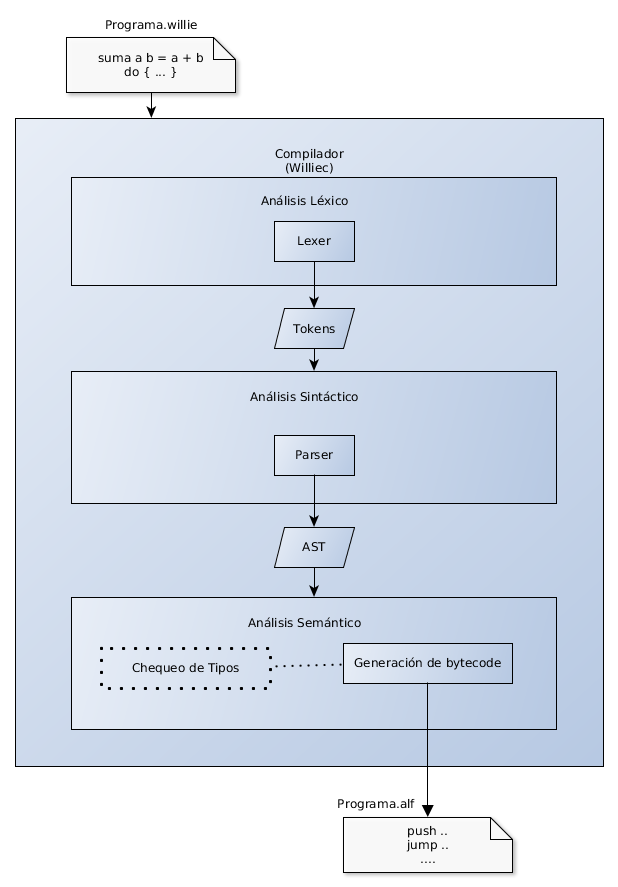
\includegraphics[width=0.9\textwidth]{graphs/compiler.png}
\label{fig:compiler}
\end{center}
\end{figure}

  TODO: Describir la Figura.

%%  El programa resultado tendrá al principio las traducción de las
%%instrucciones correspondientes al bloque \texttt{do}.
%%  Las mismas al ser ejecutadas armarán el grafo de señales del programa.
%%
%%  Al final del bloque, habrá una instrucción \texttt{halt} que cederá el
%%control al $dispatcher$.
%%
%%  Luego estará el código correspondiente a cada función definida.
%%  Cada invocación a función, tendrá la referencia directa hacia la
%%posición en el código de la misma.



  Para utilizar el compilador, dado un archivo \textit{Ejemplo.willie}, se
  ejecuta:

  \begin{verbatim}
  > williec < Ejemplo.willie > Ejemplo.alf
  \end{verbatim}

\section{Máquina virtual}

  La máquina, deberá ejecutar el código de bajo nivel en una plataforma
  objetivo.

  Existen dos limitaciones importantes a tener en cuenta, la primera es que
el espacio de memoria varía en diferentes plataformas, por lo que se desea
sea posible compilar la máquina aún con un espacio muy reducido.

  La segunda es que las plataformas varían en capacidades
de \textit{Entrada/Salida}, es importante que quien compila la máquina y
arma un entorno tenga conocimiento de cómo disponer las mismas y qué
limitaciones existen, por ejemplo: Cantidad de pines digitales o analógicos.

  La implementación modelo, se hizo utilizando
  la plataforma \textit{MBED LPC1768},
se puede encontrar documentación de la misma en \cite{mbed-LPC1768} 
y en \cite{mbed}.

  El lenguaje de programación elegido para el desarrollo de la máquina virtual
es \textit{C++} ya que es posible compilarlo para casi cualquier plataforma
objetivo.
  Además \textit{C++} permite acceder a muy bajo nivel, y manipular a
nivel de \emph{bytes} las estructuras.\\

  \textit{MBED} es una plataforma pensada para colaborar mediante
un entorno de desarrollo web, y compilador online, ese esquema de 
trabajo no es el más práctico para desarrollar la máquina virtual, por
lo que se descargaron de la página de mbed \cite{mbeddev}, las herramientas
de desarrollo para compilar offline.

TODO: Faltan muchos detalles.
TODO: Esto iría en el manual de usuario:
  El código de la máquina virtual está en el directorio
  /src/alfvm, para compilarlo se ejecuta:

\begin{verbatim}
  > cd src/alfvm
  > make
\end{verbatim}

  Ésto genera un archivo \emph{mbed\_alfvm.bin}.
  Para cargar la máquina en la placa \textit{MBED}, alcanza con conectarla
a un puerto USB y pegar el archivo en la carpeta /media/MBED.

